\subsection{Time-of-Flight Particle identification}

%Although not primarily designed for particle identification of fast
%(low-mass) particle, the MTD naturally provides some particle
%identification capability for pions, kaons and protons of \pt lower
%than a few \GeV. This capability can 
Particle identification with the MTD is based on the time-of-flight 
difference of particles with different masses and thus velocity for 
a given particle momentum, $p$:

\begin{equation}
\label{eq:tof}
\Delta t = \frac{L}{c}\left( \frac{1}{\beta_{1}} - \frac{1}{\beta_{2}}\right),
\end{equation}

\noindent where $L$ is the particle flight distance, and $\beta_1$ ($\beta_2$) 
is the velocity of particle 1 (2). 

% Figure~\ref{fig:CMS-MTD} shows the expected performance in separating 
% charged pions, kaons, and protons, as a function of transverse momentum 
% (\pt) and rapidity ($y$), in the barrel (BTL) and endcap (ETL) timing 
% layers with a time resolution of 30~ps. 
% In the barrel region, a minimal \pt\ of 0.7~GeV is required for
% particles to reach the BTL. Different colors of shaded regions correspond 
% to 2$\sigma_{T}$ and 3$\sigma_{T}$ separations. At midrapidity, proton
% identification up to \pt $\sim$ 5~GeV is achievable, while pions and 
% kaons can be separated up to \pt $\sim$ 2.5~GeV. The PID capability will 
% in general decrease toward high rapidity due to rapid increase of 
% total momentum and thus reduced time-of-flight difference. Nevertheless, 
% good performance can be still achieved over $|y|<2$.

% \begin{figure}[thb]
% \centering
% 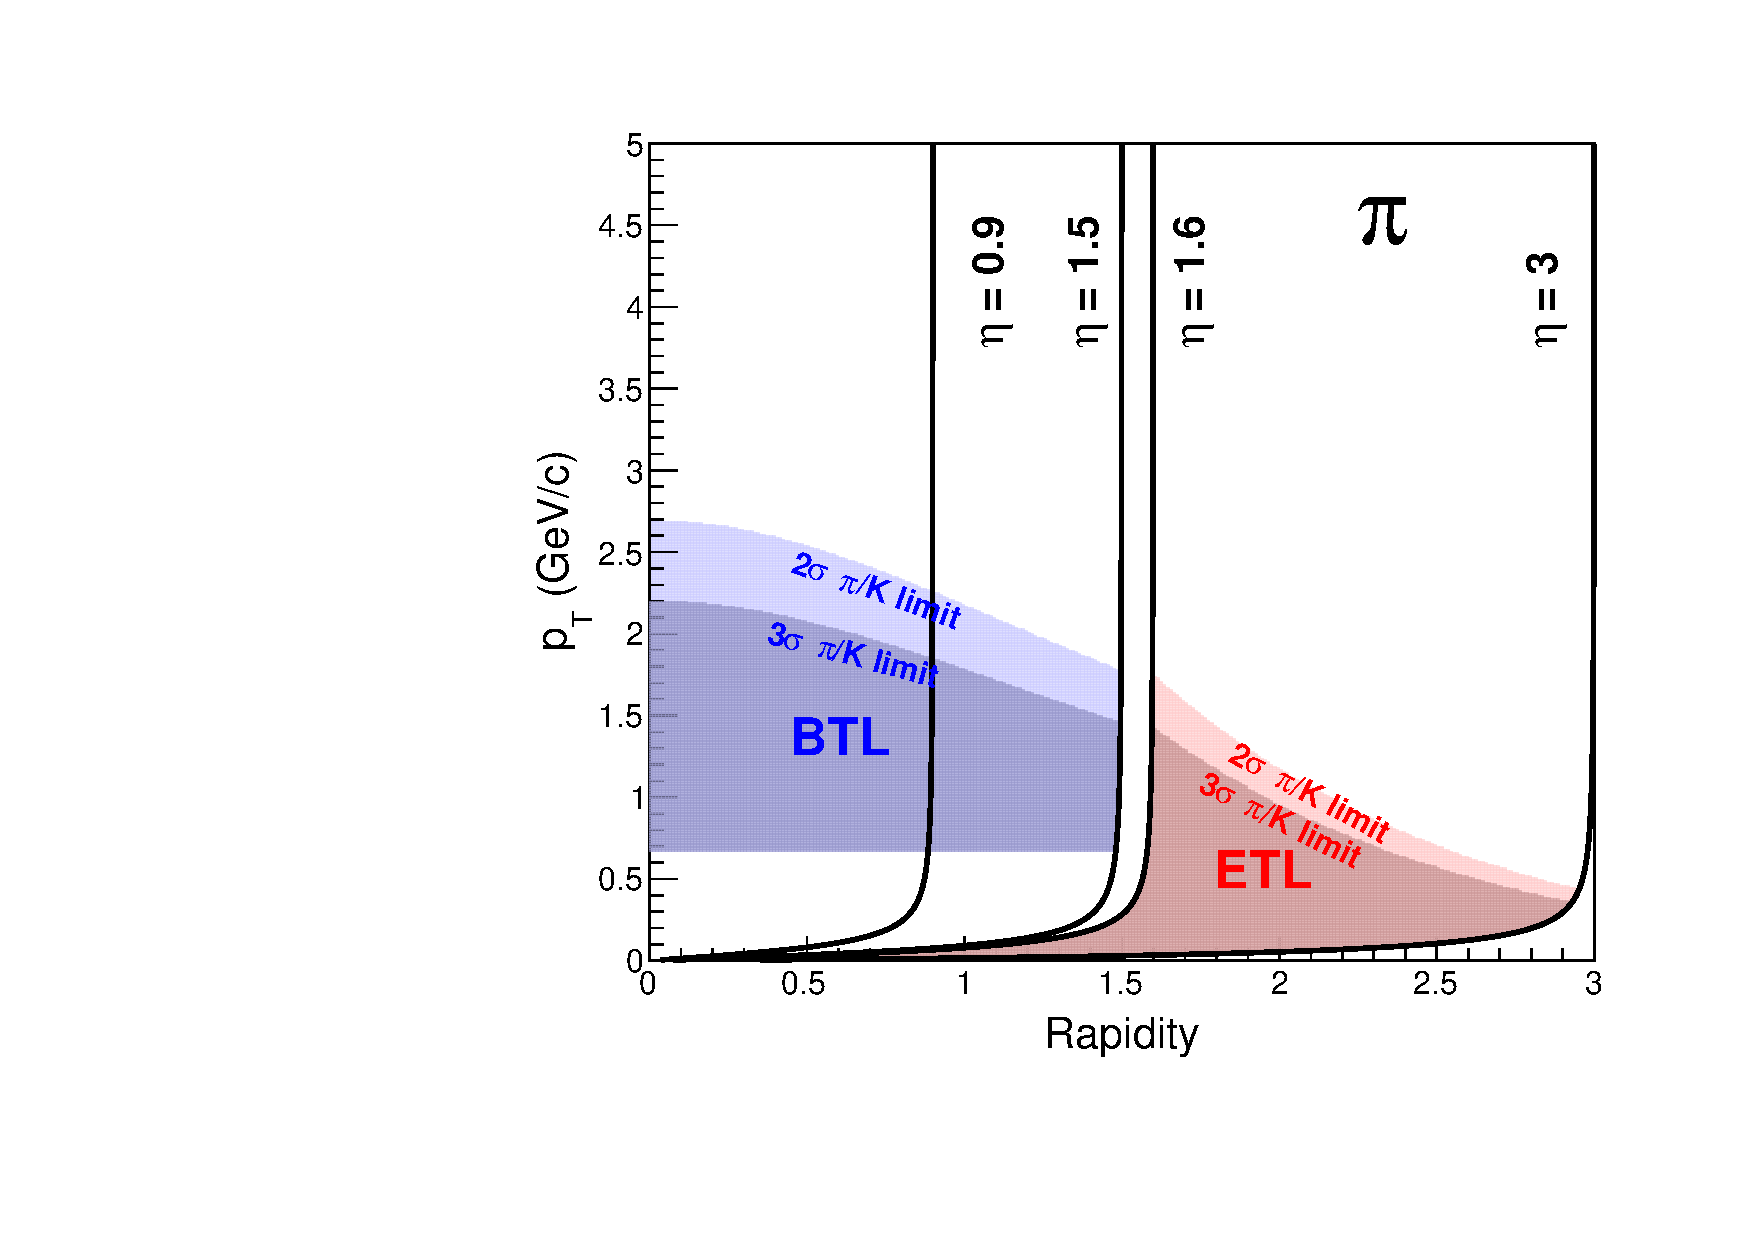
\includegraphics[width=0.49\textwidth]{fig/performance/CMSTiming_piK_30ps_NoDeDx.pdf}
% 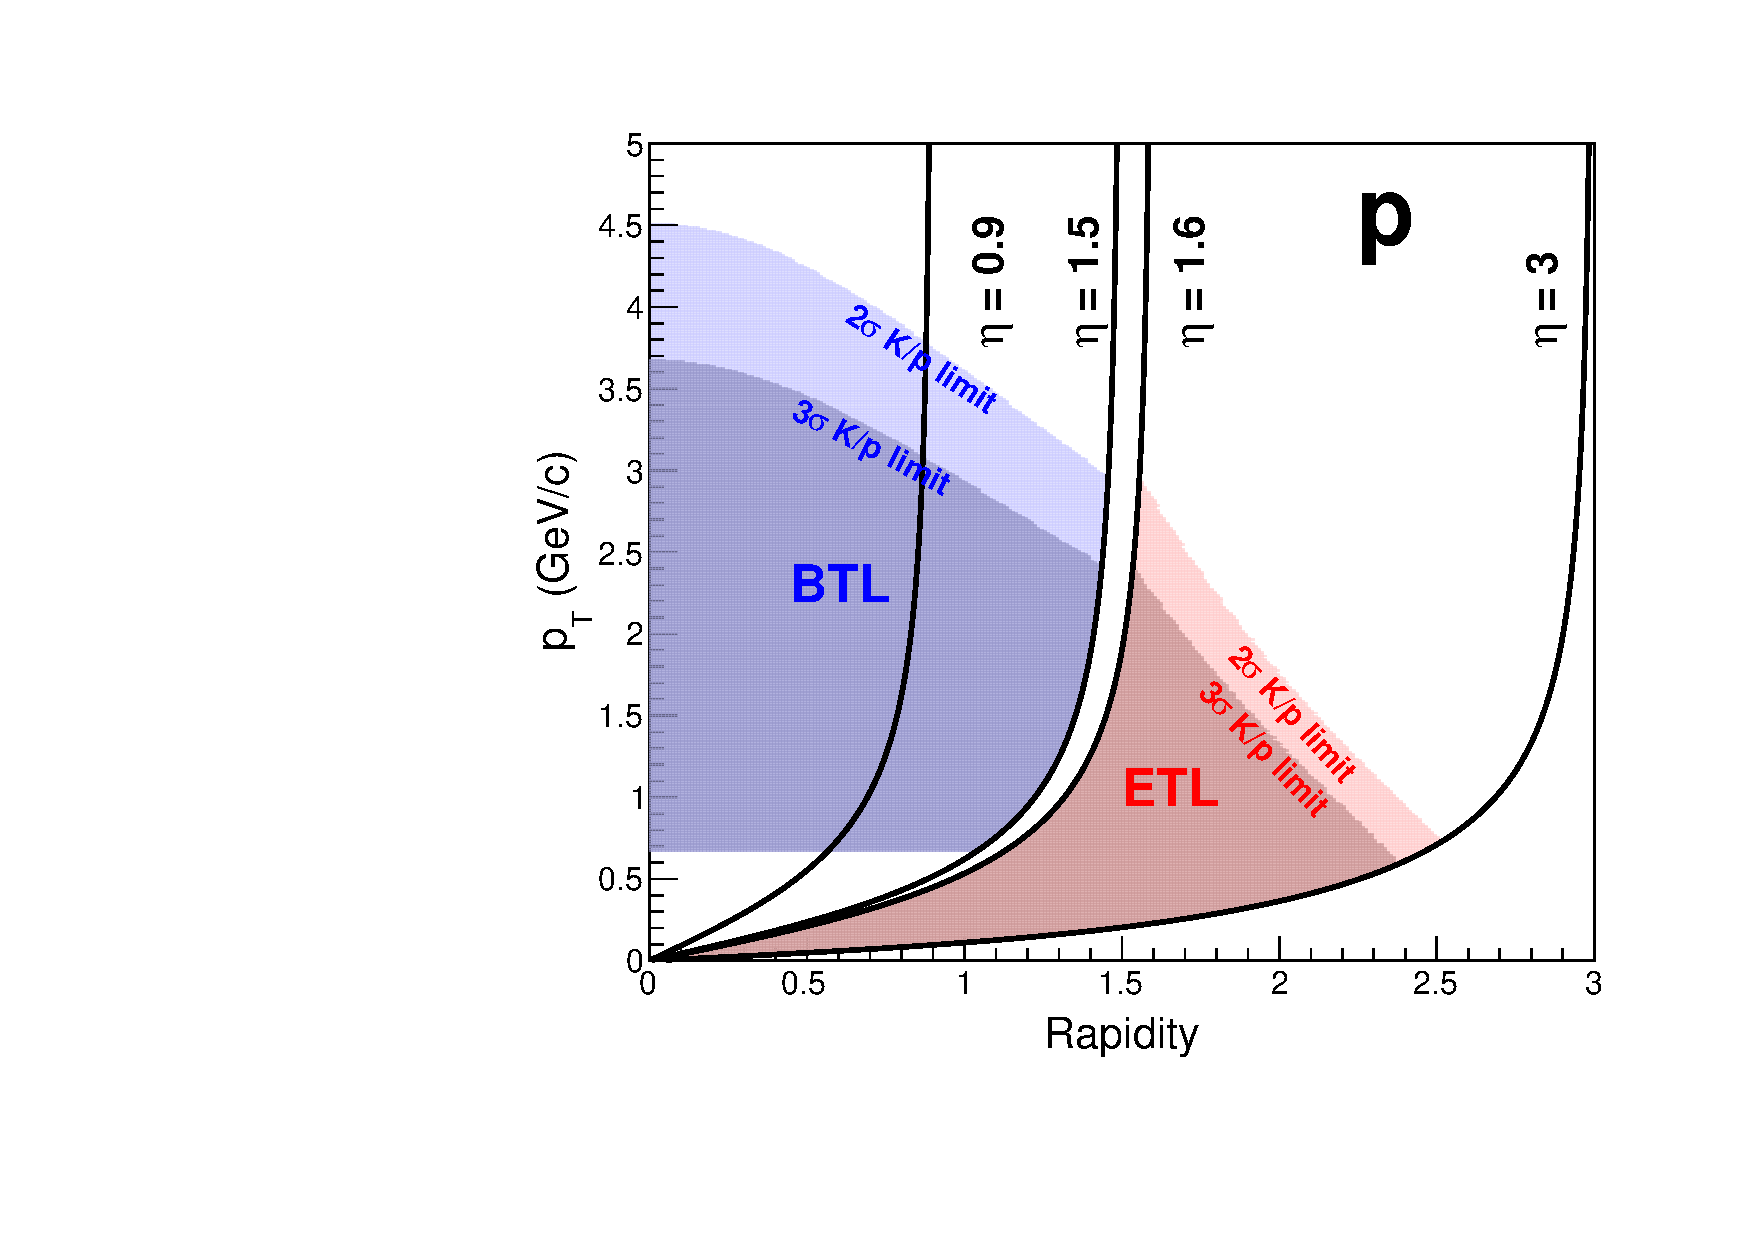
\includegraphics[width=0.49\textwidth]{fig/performance/CMSTiming_pK_30ps_NoDeDx.pdf}
% \vspace{-0.2cm}
%   \caption{ \label{fig:CMS-MTD} Expected performance of charged $\pi$/K/p
%   separation in \pt\ and rapidity with the proposed CMS-MTD in HL-LHC (Run-4),
%   with the design time resolution of 30~ps.}
% \end{figure}

% Performance of particle identification for the proposed CMS-MTD is 
% compared to that of TOF systems in the STAR and ALICE experiments at 
% midrapidity ($|y|<0.9$--1). Table~\ref{tab:tof} summarizes key parameters 
% of the TOF system in each experiment for the radius ($r$) of the 
% cylindrical barrel region, which is directly related to the particle 
% flight distance, $L$, in Eq.~\ref{eq:tof}, the time resolution ($\sigma_{T}$),
% and the ratio of $r$ to $\sigma_{T}$, which characterises the TOF PID 
% capability. Although the CMS-MTD has the shortest flight distance 
% constrained by the available space in CMS, with the design time resolution 
% of 30~ps, the PID performance is expected to be 40\% better than
% the STAR-TOF and only about 20\% worse than the ALICE-TOF in the 
% midrapidity region. More importantly, the wide acceptance of the MTD 
% provides CMS unique PID coverage to high rapidity regions.

% \begin{table}[htb]
% \centering
% \caption{\label{tab:tof} Summary of key parameters of the 
% time-of-flight system for different experiments including the radial 
% size ($r$), pseudorapidity ($\eta$) coverage, time resolution 
% ($\sigma_{T}$), and a ratio of $r$ to $\sigma_{T}$ as a measure 
% of the PID capability at midrapidity.}
% \vspace{0.2cm}
% \begin{tabular}{ c | c | c | c | c }
% \hline
% Experiment & $r$ (m) & $\eta$ coverage & $\sigma_{T}$ (ps) & $r$/$\sigma_{T}$ ($\times 100$)  \\
% \hline
% STAR & 2.2 & $|\eta|<1.0$ & 80 &  2.2 \\
% ALICE & 3.7 & $|\eta|<0.9$ & 80 &  4.6 \\
% CMS & 1.16 & $|\eta|<3.0$ & 30 &  3.9 \\
% \hline
% \end{tabular}
% \end{table}

Realistic performance of particle
identification is studied with the full CMS simulation and
reconstruction framework. Event samples are generated using the HYDJET
event generator for minimum bias PbPb collisions at 5~\TeV. 

Unlike high pileup $\Pp$$\Pp$ events, there is on average only one
PbPb collision present in each beam crossing and all particles are originated
from a well-defined reconstructed vertex in (x,y,z) coordinates. To
calculate the particle velocity, the common event start time,
$t_{0}^{\rm evt}$, is taken to  be the time of the most populated 4D
vertex, reconstructed with a pion mass hypothesis for all tracks (a
good enough approximation); the particle arrival time is provided by
the MTD hit, $t_{0}^{\rm MTD}$. The reciprocal of the particle
velocity can be calculated as:

\begin{equation}
\frac{1}{\beta}=\frac{c(t_{0}^{\rm MTD}-t_{0}^{\rm evt})}{L}.
\end{equation}

\noindent where $L$ is the path length of a track from the beam line to the MTD.

Figure~\ref{fig:betavsp} shows the 2-D distributions of
$\frac{1}{\beta}$ as a function of the particle momentum in minimum
bias HYDJET PbPb events, for the BTL and ETL regions,
respectively. The expected bands for pions, kaons and protons are
clearly visible. The resolution is consistent with the expectation,
with proton ID up to $p \sim 5$~GeV and kaon ID up to $p \sim 3$~GeV.  
%Figure~\ref{matchingeff_mtd} shows the efficiency
%for a reconstructed track to match with a MTD hit as a function of \pt and $\eta$.

\begin{figure}[thb]
\centering
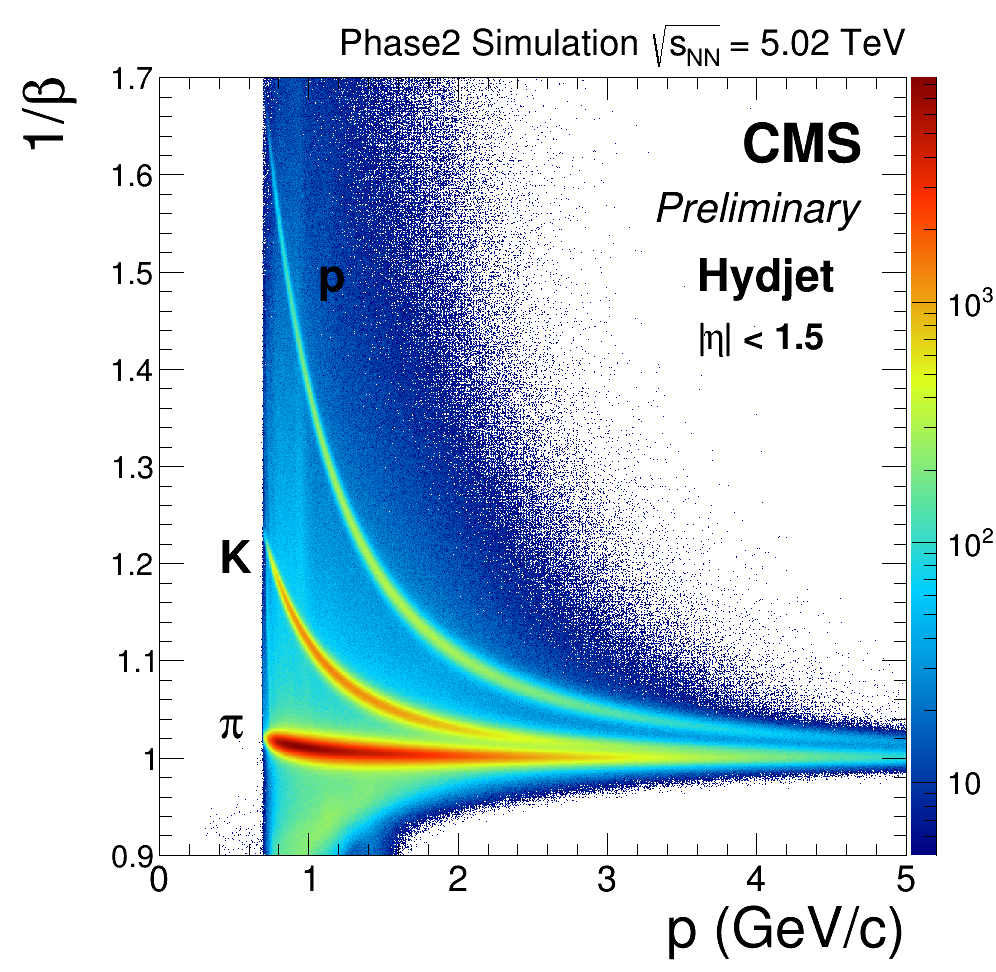
\includegraphics[width=0.48\textwidth]{fig/performance/cInvTOF_MC_Hydjet_PbPb_BTL_Inc.png}
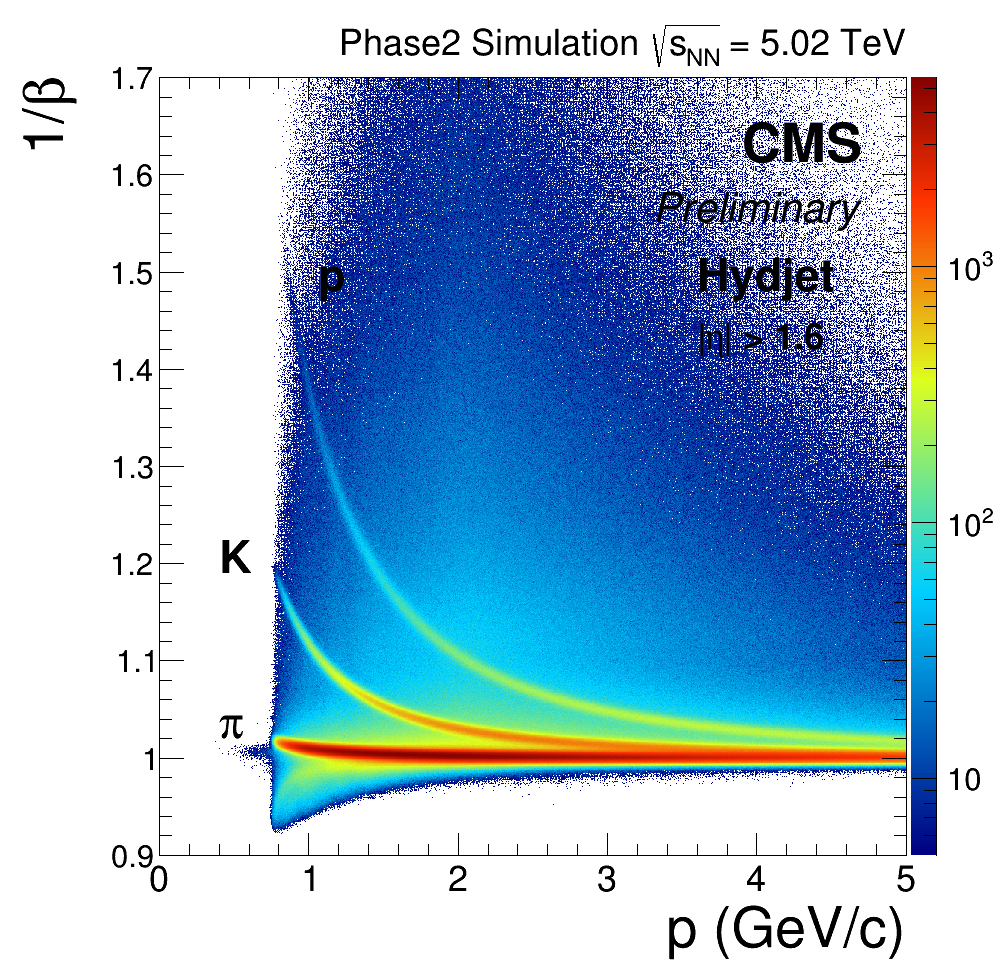
\includegraphics[width=0.48\textwidth]{fig/performance/cInvTOF_MC_Hydjet_PbPb_ETL_Inc.png}
\vspace{-0.2cm}
  \caption{ \label{fig:betavsp} The inverse velocity (1/$\beta$) as a
    function of the particle momentum, $p$, for BTL ($|\eta|<1.5$) and ETL ($|\eta|>1.6$) in HYDJET PbPb simulation at 5~\TeV.}
\end{figure}

%\begin{figure}[thb]
%\centering
%\includegraphics[width=0.6\textwidth]{fig/performance/matchingeff_mtd.pdf}
%\vspace{-0.2cm}
%  \caption{ \label{fig:matchingeff_mtd}}
%\end{figure}
%editors: W. Li & J. Bendavid & L. Gray
